\documentclass[journal,10pt]{IEEEtran}
\usepackage{amsmath,amssymb,booktabs,array,graphicx,cite,url,microtype}
\usepackage[caption=false,font=footnotesize]{subfig}
\graphicspath{{figs/}}
\newcommand{\yes}{$\checkmark$}
\newcommand{\na}{\textemdash}
\newcommand{\tp}{\mathrm{TPR}}
\newcommand{\fpr}{\mathrm{FPR}}
\newcommand{\pp}{\,pp}
\hyphenation{feder-ated general-iz-ation heterogeneous cyber-security}
\begin{document}
\title{Low-FPR Generalization Failures in Federated Intrusion Detection: A Cross-Dataset Benchmark of Ranking and Threshold Transfer}

\author{Author names and affiliations withheld for review% 
\thanks{Code and data availability are detailed at the end of the main text.}}
\maketitle
\begin{abstract}
Federated intrusion detectors must recognize attacks on a new dataset while keeping false alarms within an operational budget. We examine whether source calibration transfers, how much attack sensitivity remains when the target false-positive rate (FPR) is constrained, and whether zero-target-label calibration, linear federated models, test-time adaptation, or tail-weighted losses mitigate these failures. Across 300 native-allocation evaluations of 15 baseline methods over four held-out NetFlow datasets (with source-only selection and calibration), thresholds targeting a nominal 1\% source FPR yielded a 17.77\% mean target FPR; 285 exceeded the budget, and restoring the budget retrospectively with benign target labels yielded only 6.33\% mean recall. A source-domain tolerance rule (FedRAT) lowered mean target FPR to 7.81\% (25.5\% budget coverage) while cutting recall from 36.73\% to 15.07\%. In contrast, calibrating thresholds on 2,000 \emph{unlabeled} target flows at realistic 1\% attack prevalence reduced mean target FPR to 0.83\% (UT-Quantile, retaining 95\% of labeled-oracle recall) and 0.49\% with 97.1\% budget coverage (UT-RAT), while exposing an attack-contamination boundary once prevalence exceeds the nominal budget. Four targeted federated extensions (80 additional runs) show that federated logistic regression (FedLogReg) achieves the highest AUROC (0.753), lowest source-locked FPR (7.1\%), and highest federated 1\%-FPR recall (15.4\%); unsupervised test-time BatchNorm adaptation (FedBN\_TTA) lifts BoT-IoT 1\%-FPR recall from 0.13\% to 8.92\% (+8.80\,pp) but inflates source-locked FPR to 36.4\% unless paired with unlabeled target calibration; and source-side tail-weighted losses overfit source benign tails. Feature-level attribution traces BoT-IoT's low-FPR collapse to 109 heavy-hitter benign flows (KS 0.949--0.991). A further 1,120 evaluations test allocation and participation sensitivity. Assessing federated detectors under shift therefore requires reporting realized false-alarm rates, target-budget sensitivity, and unsupervised target-side calibration together.

\end{abstract}
\begin{IEEEkeywords}
Federated learning, intrusion detection, out-of-distribution generalization, low-FPR evaluation, domain shift, false-positive rate, calibration, client heterogeneity, benchmarking.
\end{IEEEkeywords}

\section{Introduction}
Machine-learning intrusion detection systems (IDSs) are frequently trained and validated on a single curated traffic corpus. Yet benign traffic composition, host roles, collection software, attack mixtures, and class prior probabilities change across networks. Such mismatches invalidate naive assumptions that a detector's in-domain area under the ROC curve (AUROC), accuracy, or F1 score will translate into operationally useful alarms. Sommer and Paxson warned about the gap between closed-world evaluations and deployed intrusion detection \cite{sommer2010}; later security-ML studies identified evaluation leakage, unrealistic splits, and distribution shift as recurring problems \cite{pendlebury2019,arp2022}.

Federated learning (FL) avoids directly collecting clients' raw records at one training site \cite{mcmahan2017}. This is attractive for multi-organization monitoring, but decentralized optimization introduces unequal class frequencies, domain-specific traffic signatures, intermittent participation, and communication constraints \cite{li2020,reddi2021}. More fundamentally, preserving raw data locally does \emph{not} guarantee an unseen organization's traffic will be recognized, nor does it guarantee that a threshold achieving 1\% false positives in source validation will behave similarly on a new network.

Our primary question is how much detection survives a change of dataset when the false-alarm budget stays fixed. Earlier work motivates source-calibrated alert budgets and controlled client allocations \cite{bilal2026,jin2026,khan2025}. Experiments 8--10 provide the primary NetFlow evidence; Appendix A documents the earlier fixed-schedule and attack-family studies.

\subsection*{Contributions}
\begin{itemize}
\item We benchmark 15 learners using separate source partitions for fitting, model selection, calibration and held-out source testing.
\item We compare each model's transferred operating point with its retrospective target-quantile recall, isolating the sensitivity available near the false-alarm budget.
\item We evaluate source and target budget coverage for five threshold policies, including a distributed tolerance rule that exchanges one scalar per source group.
\item We use 1,120 additional evaluations to measure allocation and participation sensitivity while retaining each method's native-selected configuration.
\item We introduce and evaluate zero-target-label unsupervised target-stream calibration (\texttt{UT-Quantile} and \texttt{UT-RAT}) across deployment prevalences $\pi\in[0\%,5\%]$, characterizing both budget control and the attack-contamination boundary when $\pi>\alpha$.
\item We evaluate four targeted federated extensions (\texttt{FedLogReg}, zero-leakage \texttt{FedBN\_TTA}, \texttt{FedAvg\_Tail}, and \texttt{FedNova\_Tail}) and trace BoT-IoT's low-FPR collapse to specific heavy-hitter benign flow features.
\item We translate conditional error rates into alert volume and precision at an assumed attack prevalence, and provide the code, manuscript sources, and domain-level results for reproduction.
\end{itemize}

\section{Related Work}
\subsection{Federated Intrusion Detection and Heterogeneous Optimization}
Early FL-IDS research established the feasibility of training security detectors without sending original traffic records to a central trainer. Ferrag \emph{et al.} benchmarked federated deep learning for IoT cybersecurity \cite{ferrag2021}; DeepFed studied industrial cyber--physical intrusion detection \cite{deepfed2021}; and 2DF-IDS combined decentralization and differential privacy for industrial IoT protection \cite{friha2023}. These papers address substantive training, privacy, and classification questions; their conclusions should not be dismissed merely because they do not report our particular set of reliability diagnostics. Djaidja \emph{et al.} compared centralized, local, and heterogeneous FL intrusion detection for 5G network slicing, reporting persistent gaps under non-IID data \cite{djaidja2024}. Reviews in \emph{Computer Networks} and \emph{Computer Science Review} document variation in FL-IDS datasets, partition policies, models, and evaluation practice \cite{belenguer2025,makris2025}.

FL optimization itself is an active source of methodological choices. FedAvg aggregates client updates \cite{mcmahan2017}, FedProx regularizes local deviations \cite{li2020}, and adaptive server optimizers such as FedAdam and FedYogi address heterogeneous optimization \cite{reddi2021}. FedNova and SCAFFOLD offer further treatments of inconsistent local objectives and client drift \cite{wang2020,karimireddy2020}. The original benchmark evaluates the first four optimizers. The tuned NetFlow extension also evaluates FedNova and SCAFFOLD. No claim is made that a single hyperparameter setting is a definitive ranking of federated optimizers.

\subsection{Cross-Dataset Generalization and Benchmark Validity}
An alternative line of research questions the evaluation data themselves. Edge-IIoTset was introduced for IoT/IIoT security experiments including federated protocols \cite{ferrag2022}. Sarhan \emph{et al.} proposed harmonized NetFlow feature families that make cross-source experimentation possible \cite{sarhan2021,sarhan2022,sarhan2022b}. However, common feature names do not ensure equivalent operational semantics or independent traffic acquisition. Duplicate records and correlated flows can make ordinary random splits substantially easier than transfer to a genuinely unseen site \cite{arp2022,pendlebury2019}. Bouke and Abdullah empirically documented how preprocessing-induced pattern leakage affects the apparent reliability of intrusion detectors \cite{bouke2023}.

Recent comparisons move beyond in-domain accuracy. Khan \emph{et al.} investigated centralized versus federated IDS under data and label skew, including client fairness and dropout \cite{khan2025}. Bilal \emph{et al.} evaluated multiple IoT datasets using FedAvg, FedProx, and FedNova, with cross-dataset and mixed-domain settings \cite{bilal2026}. An IEEE conference study specifically compared centralized and federated anomaly detection on unseen NetFlow domains \cite{softcom2026}. Other recent work evaluated unseen attacks alongside cross-dataset and leakage-sensitive protocols \cite{leakage2026}. Therefore, neither multi-dataset transfer nor auditing alone is new here. Our narrower claimed distinction is the \emph{joint, source-locked, low-FPR and alert-budget evaluation} of FL under additional controlled client allocation perturbations.

\subsection{Unknown Attacks, Drift, and Threat-Specific Evaluation}
Unknown-attack and unknown-network testing are conceptually different. Open-set recognition methods distinguish known semantic categories from genuinely novel categories \cite{bendale2016}; in an IDS, a binary classifier can still assign the label ``attack'' to a family omitted from training. It would therefore be misleading to present our binary held-out-family experiment as a full open-set multiclass recognition system. Similarly, held-out-source evaluation does not guarantee temporal robustness: actual traffic may change inside the same network. Yang \emph{et al.} study self-supervised concept-drift adaptation in network intrusion detection \cite{yang2025}, whereas our protocol intentionally prohibits post-deployment adaptation using target labels. This makes our estimates strict zero-target-label transfer results, not a replacement for adaptive detectors.

Evaluation also depends on how attack families, nuisance variables, and flow records are constructed. Sharafaldin \emph{et al.} emphasize traffic characterization when creating an intrusion detection dataset \cite{sharafaldin2018}; subsequent benchmark critiques identify leakage due to repeated, overlapping, or temporally entangled examples \cite{arp2022,pendlebury2019}. Our fingerprint analysis is a limited but explicit check against this risk. It is used to qualify interpretability, not to assert that all collection artifacts have been eliminated.

\subsection{Decision Thresholds, Calibration, and Alert Costs}
AUROC integrates over thresholds that an operator may never use. For rare attacks, precision can be sharply reduced by small false-positive probabilities \cite{saito2015}. Neural confidence is not intrinsically calibrated \cite{guo2017}, and calibration can degrade under dataset shift \cite{ovadia2019}. Jin and Lee recently combined cross-dataset evaluation, source calibration, score-orientation diagnostics, and alert budgets in a \emph{non-federated} IDS setting \cite{jin2026}; this is a direct conceptual neighbor of our operational analyses and is explicitly acknowledged rather than presented as an unfilled gap. Our experiments extend that question to a fixed FL-versus-central-versus-local comparison, four held-out NetFlow sources, and client heterogeneity interventions. The prevalence adjustment is a \emph{counterfactual base-rate calculation}, not a measured traffic experiment \cite{lipton2018}.

\section{Study design and methods}
\subsection{Primary NetFlow protocol (Exps.~8--10)}
The harmonized NetFlow reference sample contains 96,000 flows and 41 features. The fingerprint filter retains one representative of each within-domain, same-label and same-family feature signature and excludes signatures shared across domains or assigned conflicting labels or families. This leaves 93,810 flows. Exp.~8 uses four dataset holdouts and five seeds. Within the sources, separate partitions serve fitting, early stopping, calibration and testing. Each method receives four candidate configurations. Selection maximizes mean inner held-out-source standardized partial AUROC up to 5\% FPR. Federated training permits 150 rounds. Table~\ref{tab:primary} lists all 15 methods. The eight allocation comparators are LocalMLP, FedAvg, FedProx, FedAdam, FedYogi, FedNova, SCAFFOLD and the FedBN source ensemble. Exp.~9 applies native, quantity and label allocations at two-thirds participation, plus mixed, quantity, label and domain allocations at full participation. Reusing native settings measures sensitivity at a fixed configuration.

The NetFlow v2 source datasets and original schema are documented by Sarhan et al.~\cite{sarhan2022}. Source-domain identifiers define the clients in the native allocation and are excluded from the 41 predictors. Within each source we allocate approximately 70\% to fit and 10\% each to stopping, calibration and source test. Seeds are 0, 42, 123, 2026 and 3407. The standard MLP uses 41--64--32--1 units with ReLU hidden activations. Binary cross-entropy uses logits. The source-fit standardizer follows a fixed signed-log transform. Eight local steps use batches up to 256. Source stopping pAUC is checked every five rounds with patience ten checks and minimum 30 rounds. 

\emph{Candidate grids.} Logistic regression uses $C=0.01,0.1,1,10$. Random Forest uses 300 trees with (depth, minimum leaf size) equal to (12,1), (unlimited,1), (16,5), (unlimited,5). LightGBM uses up to 1,500 trees, stopping after 50 rounds without source-validation improvement, with (learning rate, leaves) equal to (.03,31), (.1,31), (.03,63), (.1,63). Neural candidates use learning rates .0003, .001, .003 and .01, except SCAFFOLD (.001, .003, .01, .03) and FedProx, whose (rate, $\mu$) pairs are (.001,.001), (.001,.01), (.01,.001), (.01,.01). FedAdam and FedYogi use (local rate, server rate) pairs (.001,.01), (.001,.05), (.003,.01), (.003,.05), with $\tau=.01$. Equal candidate counts do not imply equal resource costs.

GroupDRO reweights source groups multiplicatively using loss coefficient 0.05~\cite{sagawa}. CORAL penalizes pairwise source hidden-covariance discrepancies with weight 0.1~\cite{coral}. DANN uses source group labels in a gradient-reversed linear head weighted 0.1~\cite{dann}. These three baselines pool source features. The FedBN adaptation keeps batch normalization local at both hidden layers and averages source-model scores on the unseen dataset~\cite{fedbn}. No target batch statistics enter inference.

Exp.~10 applies five thresholds to each frozen score vector. The federated risk-aware threshold (FedRAT) implements a nonparametric tolerance limit~\cite{wilks}. Each source group can transmit one scalar upper threshold (three float64 values, 24 payload bytes in the native federation). This statistic may disclose information about rare benign scores. The simulation provides neither encryption nor differential privacy. Conformal order statistics rely on exchangeability~\cite{vovk}. For the tolerance rule, order the benign calibration scores in source group $j$ as $s_{j,(1)},\ldots,s_{j,(n_j)}$. With $J$ groups, $\delta=0.05$ and nominal FPR $\alpha$, set
\[
 k_j=1+Q_{1-\delta/J}\{\mathrm{Binomial}(n_j,1-\alpha)\}.
\]
Here $Q$ is the smallest integer reaching the specified cumulative probability. Flag scores strictly above $\max_j s_{j,(k_j)}$, taking the threshold as infinity if an index exceeds its group size. The order-statistic calculation assumes independent draws within each source group. The multiplicity adjustment covers those groups and imposes no bound on a shifted target. Pooled empirical and conformal rules use the combined benign sample. Minimax empirical and worst-source conformal take the largest corresponding source-group threshold. For a given fitted model all five policies share one ROC curve. We therefore report a common retrospective target-quantile recall at nominal 1\% FPR (ties may lower achieved FPR), alongside the operating points selected without target labels. Fig.~\ref{fig:pipeline} summarizes the complete source-locked evaluation pipeline, including the zero-target-label target-stream calibration branch and the four federated extensions described below.

\begin{figure*}[t]\centering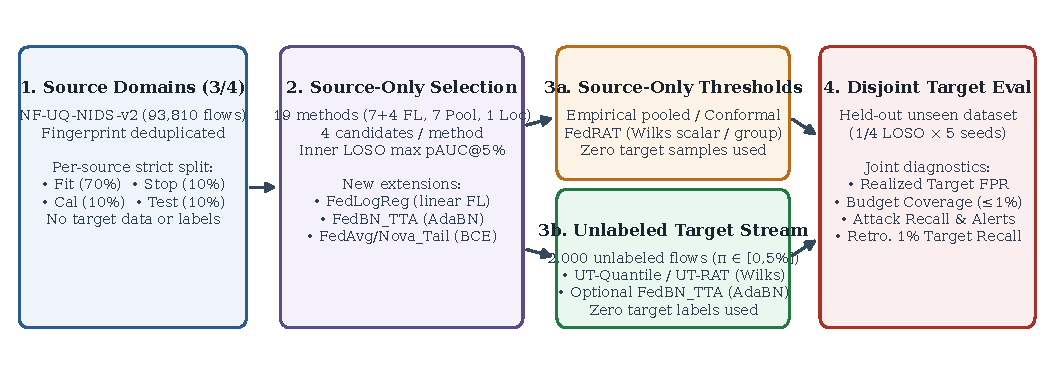
\includegraphics[width=\textwidth]{protocol_pipeline.pdf}
\caption{Overview of the source-locked FLIDS evaluation protocol. Source datasets are strictly partitioned for fitting, early stopping, calibration, and source testing; target labels never enter training, model selection, feature scaling, or threshold calibration. Unlabeled target-stream calibration (\texttt{UT-Quantile}/\texttt{UT-RAT}) and optional unsupervised BatchNorm adaptation (\texttt{FedBN\_TTA}) operate on a disjoint unlabeled target stream before held-out evaluation.}\label{fig:pipeline}\end{figure*}

\emph{Zero-target-label target-stream calibration and federated extensions.} In operational monitoring, an organization observes an \emph{unlabeled} stream $U$ of local target flows whose true attack prevalence $\pi$ is typically low. Applying the empirical $(1-\alpha)$ quantile (\texttt{UT-Quantile}) or the one-sided binomial tolerance limit with $\delta=0.05$ (\texttt{UT-RAT}) directly to $s(U)$ requires zero target labels. Because $U$ is a mixture $(1-\pi)P_0+\pi P_1$, matching total alert rate $(1-\pi)\fpr(\tau)+\pi\tp(\tau)=\alpha$ implies $\fpr(\tau)=(\alpha-\pi\tp(\tau))/(1-\pi)\le\alpha/(1-\pi)$, bounding benign false positives near or below $\alpha$ whenever $\pi$ is small, while higher prevalence ($\pi>\alpha$) pushes $\tau$ upward via attack contamination. We evaluate $N_{\mathrm{cal}}=2{,}000$ unlabeled target flows across $\pi\in\{0\%,0.1\%,0.5\%,1\%,2\%,5\%\}$ over five disjoint draws per run. In addition, we evaluate four targeted federated methods (80 runs across the exact same four folds, five seeds, split digests, and four-candidate inner selection): (i)~\texttt{FedLogReg}, a federated linear model (\texttt{Linear(41,1)}) with Adam weight decay grid $(0.01,10^{-2}),(0.01,10^{-3}),(0.03,10^{-3}),(0.03,10^{-4})$; (ii)~\texttt{FedBN\_TTA}, which adapts BatchNorm running statistics via label-free, gradient-free forward passes (AdaBN) on a disjoint 2,000-flow unlabeled target stream at $\pi=1\%$ (evaluated strictly on the remaining held-out target flows, alongside paired pre-TTA scores); and (iii)~\texttt{FedAvg\_Tail} and \texttt{FedNova\_Tail}, which replace standard BCE with an asymmetric negative-tail focal loss weighting benign flows ($y=0$) by $1+\lambda\sigma(z)^2$ with $\lambda\in\{2,5\}$ to penalize high-scoring source benign records.

\section{Experimental results}

\begin{table*}[t]\centering\small
\caption{Native allocation and full participation. Mean $\pm$ sample SD over four dataset means, each averaged over five seeds. Partial AUC is standardized to 1\% FPR. The last three columns are percentages.}\label{tab:primary}
\begin{tabular}{lrrrrrr}\toprule
Method & Training & AUROC & pAUC & Locked FPR & Locked recall & Target-quantile recall\\\midrule
CORAL & Pooled & 0.617 $\pm$ 0.161 & 0.502 $\pm$ 0.003 & 24.4 $\pm$ 9.3 & 35.0 $\pm$ 16.2 & 1.5 $\pm$ 1.1\\
DANN\_Source & Pooled & 0.636 $\pm$ 0.174 & 0.507 $\pm$ 0.006 & 23.6 $\pm$ 8.0 & 42.2 $\pm$ 26.0 & 2.0 $\pm$ 2.2\\
FedAdam & FL & 0.649 $\pm$ 0.157 & 0.509 $\pm$ 0.011 & 18.0 $\pm$ 8.7 & 34.1 $\pm$ 12.3 & 4.4 $\pm$ 4.7\\
FedAvg & FL & 0.709 $\pm$ 0.154 & 0.520 $\pm$ 0.025 & 16.3 $\pm$ 5.4 & 40.4 $\pm$ 20.6 & 9.0 $\pm$ 10.9\\
FedBN\_SourceEnsemble & FL & 0.671 $\pm$ 0.148 & 0.530 $\pm$ 0.031 & 12.0 $\pm$ 1.3 & 37.4 $\pm$ 22.7 & 8.8 $\pm$ 8.3\\
FedNova & FL & 0.713 $\pm$ 0.111 & 0.555 $\pm$ 0.098 & 7.3 $\pm$ 5.3 & 25.8 $\pm$ 28.6 & 14.8 $\pm$ 22.9\\
FedProx & FL & 0.654 $\pm$ 0.132 & 0.506 $\pm$ 0.008 & 20.2 $\pm$ 7.7 & 37.3 $\pm$ 15.0 & 2.4 $\pm$ 2.5\\
FedYogi & FL & 0.650 $\pm$ 0.167 & 0.506 $\pm$ 0.009 & 18.4 $\pm$ 8.9 & 34.0 $\pm$ 11.9 & 3.0 $\pm$ 3.1\\
GroupDRO & Pooled & 0.606 $\pm$ 0.150 & 0.503 $\pm$ 0.009 & 21.7 $\pm$ 9.7 & 30.9 $\pm$ 17.0 & 2.0 $\pm$ 2.5\\
LightGBM & Pooled & 0.636 $\pm$ 0.184 & 0.504 $\pm$ 0.009 & 23.6 $\pm$ 11.5 & 40.1 $\pm$ 18.0 & 1.6 $\pm$ 2.1\\
LocalMLP & Local & 0.689 $\pm$ 0.179 & 0.533 $\pm$ 0.030 & 8.5 $\pm$ 4.4 & 25.7 $\pm$ 26.0 & 10.6 $\pm$ 7.1\\
LogisticRegression & Pooled & 0.675 $\pm$ 0.225 & 0.573 $\pm$ 0.119 & 9.4 $\pm$ 10.0 & 46.0 $\pm$ 36.2 & 18.2 $\pm$ 26.9\\
PooledMLP & Pooled & 0.616 $\pm$ 0.128 & 0.501 $\pm$ 0.004 & 23.9 $\pm$ 7.8 & 31.8 $\pm$ 12.6 & 1.5 $\pm$ 1.4\\
RandomForest & Pooled & 0.656 $\pm$ 0.200 & 0.500 $\pm$ 0.004 & 29.1 $\pm$ 13.8 & 59.7 $\pm$ 24.9 & 0.6 $\pm$ 0.9\\
SCAFFOLD & FL & 0.665 $\pm$ 0.154 & 0.554 $\pm$ 0.096 & 10.1 $\pm$ 9.0 & 30.4 $\pm$ 26.7 & 14.5 $\pm$ 23.1\\
\bottomrule\end{tabular}\end{table*}
Table~\ref{tab:primary} shows why overall ranking, alert burden and tail sensitivity must be read together. Across all 300 runs mean target-quantile recall at the nominal 1\% budget was 6.33\%. Random Forest recovered 59.7\% of attacks at its source-locked threshold, with 29.1\% target FPR. Restoring the nominal budget reduced its recall to 0.6\%. Logistic regression, FedNova and SCAFFOLD retained 18.2\%, 14.8\% and 14.5\% recall, respectively, with substantial between-dataset dispersion. The three pooled source-generalization variants retained only 1.5--2.0\%, close to the pooled MLP's 1.5\%. An exact two-sided sign test on four nonzero paired dataset means cannot yield a $p$-value below 0.125, even if all signs agree. Table~\ref{tab:budgetsfull} gives the paired recall differences and the sensitivity at four target budgets.

\subsection{Federated, centralized and local training}
\begin{table}[t]\centering\footnotesize
\caption{Equally weighted method means by training paradigm, calculated before rounding. FPR uses the source-locked threshold; tail recall uses the nominal 1\% target budget.}\label{tab:families}
\setlength{\tabcolsep}{2.5pt}\begin{tabular}{lrrrrr}\toprule
Training & Methods & AUROC & pAUC$_{.01}$ & FPR (\%) & Tail recall (\%)\\\midrule
Federated & 7 & .673 & .526 & 14.61 & 8.13\\
Centralized & 7 & .635 & .513 & 22.24 & 3.92\\
Local ensemble & 1 & .689 & .533 & 8.54 & 10.64\\\bottomrule
\end{tabular}\end{table}
Across the seven federated methods, mean target-quantile recall was 8.13\%, compared with 3.92\% across the seven centralized methods (Table~\ref{tab:families}). The local ensemble alone attained 10.64\%, with a lower transferred FPR than either group mean. The spread of individual operating points in Fig.~\ref{fig:tunedpoints} shows how much a group average conceals. Architectures, objectives and optimizers differ within and between groups; these averages cannot isolate an effect of federated aggregation.

\begin{figure*}[t]\centering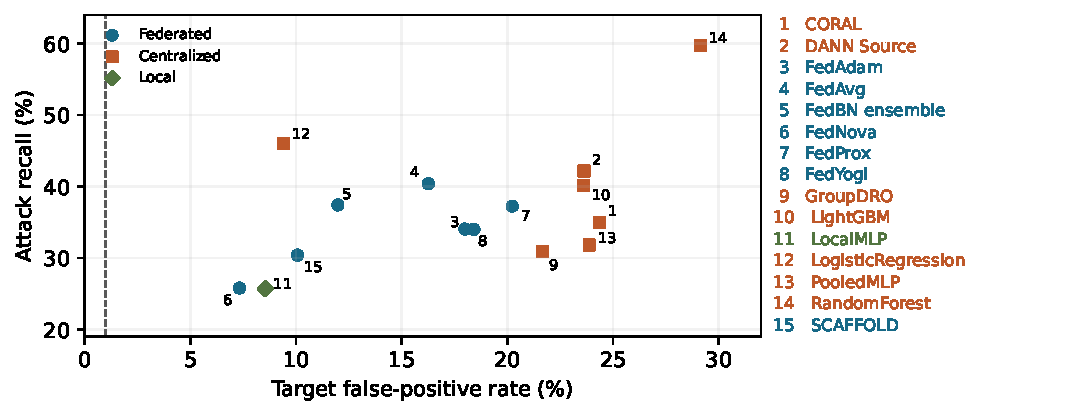
\includegraphics[width=.85\textwidth]{tuned_operating.pdf}
\caption{Source-locked operating points for all 15 tuned methods. Each point averages four held-out datasets and five seeds. The dashed line marks the nominal 1\% source calibration FPR. Target FPR varies across methods, so vertical differences do not measure recall at a matched target budget.}\label{fig:tunedpoints}\end{figure*}

Across the 15 method means, Pearson correlation between locked target FPR and target-quantile recall was $-0.918$. Both statistics depend on target benign scores, and the methods share four targets. The association describes this benchmark; it does not identify a common causal mechanism.

For each of 15 methods, four held-out domains, and five seeds, we locked the threshold using the upper 1\% tail of benign source calibration scores. Recalculation from the archived scores gave a target FPR above 1\% in 285 of 300 configurations. The same source thresholds exceeded the nominal rate on the reserved source test in 174/300 runs (58.0\%), compared with 285/300 (95.0\%) on targets. Target holdouts contained 11,953--11,992 benign records. In 284 runs the lower endpoint of the two-sided 95\% exact binomial interval exceeded 1\%. These descriptive intervals assume independent flows and do not adjust for multiple comparisons. The exceedance fraction describes repeated evaluations on four datasets; it does not estimate a probability over future sites.

\begin{figure*}[t]
\centering
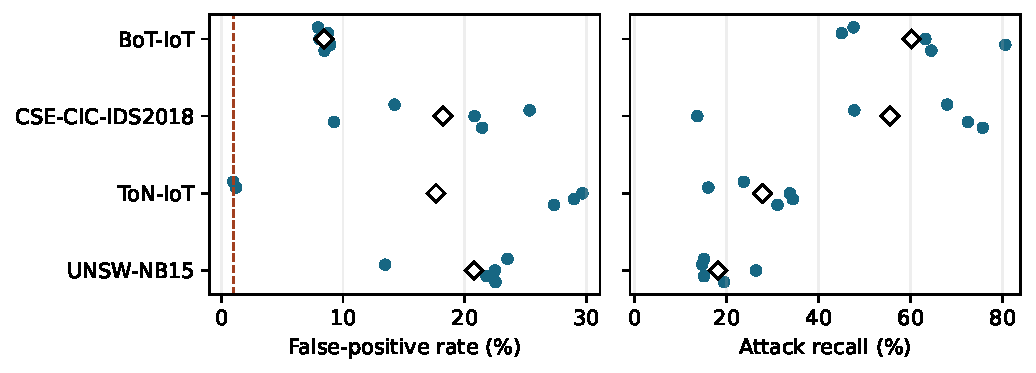
\includegraphics[width=.83\textwidth]{threshold_transfer.pdf}
\caption{FedAvg under full participation with a source-locked threshold. Each dot represents one seed and each open diamond the five-seed mean. The dashed line marks the nominal 1\% FPR. On ToN-IoT, two runs operated near the nominal rate while three exceeded 27\%.}
\label{fig:tunedtransfer}
\end{figure*}

For FedAvg, mean source-test FPR ranged from 0.96\% to 1.09\% across holdouts. In Fig.~\ref{fig:tunedtransfer}, mean target FPR rose to 8.44\%, 18.22\%, 17.64\%, and 20.76\% in the displayed domain order. Corresponding recalls were 60.19\%, 55.49\%, 27.79\%, and 18.15\%. On CSE-CIC-IDS2018, logistic regression achieved 60.21\% recall at 2.18\% FPR, improving both observed rates over FedAvg.

\begin{figure*}[t]\centering
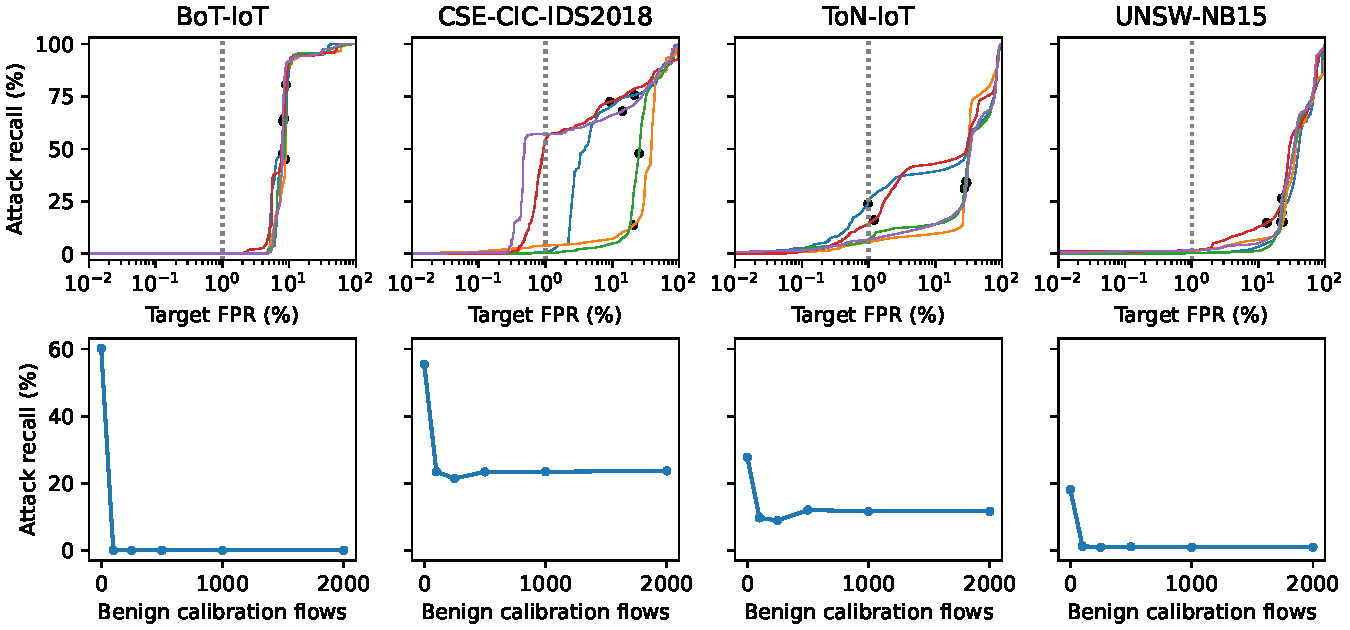
\includegraphics[width=.95\textwidth]{tail_calibration.pdf}
\caption{FedAvg on the four held-out datasets. Top: target ROC curves for five seeds, with nominal 1\% FPR marked. Bottom: recall after target-benign threshold calibration, averaged over five draws per seed. Zero uses the source threshold. Separate target-benign records evaluate false positives. Black dots show the empirical source-locked point for each seed. Both axes in the ROC panels are percentages.}\label{fig:tail}\end{figure*}

Figure~\ref{fig:tail} overlays the points from Fig.~\ref{fig:tunedtransfer} on the same per-seed ROC curves. Replaying all 300 thresholds reproduced both archived rates. On ToN-IoT, seeds 0 and 42 selected learning rate 0.0003; seeds 123, 2026 and 3407 selected 0.010, 0.003 and 0.001. Median FedAvg FPR was 27.35\% (IQR 1.20--28.99\%). This association does not isolate candidate selection from other seed-dependent changes.

\emph{Cost of restoring the operating point.} On BoT-IoT, FedAvg achieved mean AUROC 0.904. Recalibrating its threshold with 2,000 labeled benign target flows reduced FPR to 1.01\% on separate benign target flows, but attack recall fell to 0.023\%. On CSE-CIC-IDS2018 the same procedure yielded 1.12\% FPR and 23.72\% recall. These estimates average five calibration draws per seed and five seeds. The source-only FedRAT tolerance-bound prototype yielded FPR/recall of 6.46\%/27.73\% on BoT and 1.49\%/25.49\% on CSE. On BoT-IoT the near-zero recall after target calibration indicates poor ranking in the low-FPR tail despite the high overall AUROC. The tolerance rule reduced false alerts at a measurable detection cost and left both mean target FPRs above nominal.

\subsection{Client Allocation and Threshold Policy in the Tuned Benchmark}
Across Exps.~8--10, the completed NetFlow evaluation contains 1,420 model and analysis bundles. The 300 native runs cover 15 methods, four held-out datasets, and five seeds. Experiment~9 adds 1,120 matched runs by applying seven allocation or participation settings to eight methods, using the configuration selected for the corresponding native run.

For FedAvg, reducing native participation from all clients to two thirds increased mean target recall from 40.40\% to 45.72\%, alongside an increase in target FPR from 16.26\% to 18.95\%. Under full participation, the label-skew allocation yielded 46.83\% recall and 13.95\% FPR. Thus the recall loss under label skew in the earlier fixed-schedule experiment did not recur under the tuned protocol. Several training and allocation choices differ between protocols, so the reversal cannot be attributed to tuning alone.


\begin{table*}[t]\centering\small
\caption{Policy diagnostics at $\alpha=1\%$. Coverage is the percentage of 300 runs with measured FPR at or below budget. The final column is mean absolute log target-FPR ratio, with a half-count correction $(FP+0.5)/(n+1)$ to include zero counts.}\label{tab:nfpolicies}
\begin{tabular}{lrrrrr}\toprule
Policy & Source coverage & Target coverage & Target FPR (\%) & Recall (\%) & Log error\\\midrule
FedRAT & 100.00 & 24.67 & 7.81 & 15.07 & 1.80\\
empirical pooled & 42.00 & 5.00 & 17.77 & 36.73 & 2.61\\
minimax empirical & 97.33 & 9.33 & 13.81 & 28.61 & 2.33\\
pooled conformal & 47.33 & 5.00 & 17.56 & 36.34 & 2.60\\
worst source conformal & 98.33 & 10.67 & 13.21 & 27.11 & 2.27\\
\bottomrule\end{tabular}\end{table*}


\emph{FedRAT reliability and sensitivity.} On identical scores, switching from pooled empirical calibration to FedRAT reduced mean target FPR by 9.96 percentage points (approximately 56\% relative) and reduced recall by 21.66 points (approximately 59\% relative). The fraction of runs meeting the empirical budget rose by 58 points on the pooled source test and 19.67 points on targets (Table~\ref{tab:nfpolicies}). Both changes follow from moving the threshold on a fixed score vector.

On pooled source-test records the tolerance rule met the empirical 1\% budget in all 300 evaluations. Reconstructing the thresholds from the unrounded calibration scores gave 891/900 individual source-group test FPRs at or below budget. All three source groups met budget together in 291/300 fits (97.0\%), versus 74/300 held-out targets (24.7\%). This checks empirical source behavior; repeated tests on the same four datasets cannot validate a 95\% simultaneous population guarantee. Table~\ref{tab:nfpolicies} measures the size and frequency of target deviations independently of recall.

The matched control for label skew is the full-participation mixed allocation: both redistribute each source across clients. Relative to mixed, label skew raised FedAvg AUROC from 0.639 to 0.753, standardized partial AUC from 0.517 to 0.529 and target-quantile recall from 5.30\% to 12.49\%. Locked FPR fell from 21.62\% to 13.95\%. These paired operating and ranking summaries describe the chosen native hyperparameters; retuning each allocation would estimate a different effect.

\begin{table*}[t]\centering\small
\caption{Tail sensitivity and projected alert volume for the tuned methods. Columns 2--5 report attack recall (\%) at retrospective target FPR budgets. $\Delta$ is the paired difference in recall from FedAvg at the 1\% target budget (percentage points), averaged over matched datasets and seeds. The final columns instead use the source-locked threshold and assume 1\% attack prevalence; precision is averaged over runs.}\label{tab:budgetsfull}
\begin{tabular}{lrrrrrrr}\toprule
Method & 0.1\% FPR & 1\% FPR & 5\% FPR & 10\% FPR & $\Delta$ & Alerts/100,000 & Precision (\%)\\\midrule
CORAL & 0.24 & 1.47 & 10.85 & 17.77 & -7.50 & 24,464 & 1.99\\
DANN Source & 0.20 & 2.02 & 13.82 & 25.21 & -6.95 & 23,812 & 2.48\\
FedAdam & 0.41 & 4.44 & 15.06 & 30.44 & -4.53 & 18,150 & 2.86\\
FedAvg & 0.53 & 8.97 & 17.43 & 40.88 & +0.00 & 16,505 & 4.54\\
FedBN SourceEnsemble & 4.11 & 8.76 & 30.21 & 40.76 & -0.22 & 12,238 & 5.00\\
FedNova & 5.38 & 14.77 & 23.68 & 39.68 & +5.79 & 7,514 & 4.00\\
FedProx & 0.47 & 2.42 & 12.62 & 22.26 & -6.55 & 20,406 & 2.38\\
FedYogi & 0.43 & 2.99 & 15.01 & 29.19 & -5.98 & 18,576 & 2.68\\
GroupDRO & 0.47 & 2.04 & 12.85 & 18.40 & -6.94 & 21,750 & 1.74\\
LightGBM & 0.91 & 1.59 & 7.69 & 22.46 & -7.38 & 23,772 & 2.09\\
LocalMLP & 2.40 & 10.64 & 24.79 & 37.74 & +1.66 & 8,715 & 5.77\\
LogisticRegression & 3.51 & 18.20 & 40.31 & 50.63 & +9.23 & 9,795 & 10.00\\
PooledMLP & 0.16 & 1.51 & 11.46 & 17.10 & -7.47 & 23,956 & 1.71\\
RandomForest & 0.46 & 0.59 & 10.78 & 23.78 & -8.39 & 29,452 & 2.93\\
SCAFFOLD & 4.47 & 14.55 & 22.57 & 37.85 & +5.57 & 10,276 & 4.27\\
\bottomrule\end{tabular}\end{table*}
\subsection{Alerts under assumed prevalence}
For attack prevalence $\pi$, expected alerts per 100,000 flows are $10^5[(1-\pi)\mathrm{FPR}+\pi\mathrm{TPR}]$. With $\pi=1\%$, the primary FedAvg scores imply 16,505 alerts and about 404 detected attacks per 100,000 flows. Precision from the aggregate expected counts is 2.45\%; the equally weighted mean of the 20 individual precision values is 4.54\%. The first weights runs by alert volume. Neither estimates observed production prevalence. Table~\ref{tab:budgetsfull} gives the corresponding estimates for all 15 methods.
\subsection{Zero-target-label target-stream calibration}
\begin{table}[t]\centering\footnotesize
\caption{Zero-target-label calibration across unlabeled-stream attack prevalence $\pi$ ($N_{\mathrm{cal}}=2{,}000$, $\alpha=1\%$, five disjoint draws across 300 native runs). Coverage is the percentage of evaluations with target $\fpr\le 1\%$.}\label{tab:utcal}
\setlength{\tabcolsep}{2.3pt}\begin{tabular}{@{}lrrrrr@{}}\toprule
Policy & $\pi$ (\%) & FPR (\%) & Cov. (\%) & Recall (\%) & Log err.\\\midrule
Source empirical & 1.0 & 17.77 & 4.87 & 36.73 & 2.61\\
FedRAT (source) & 1.0 & 7.81 & 25.53 & 15.07 & 1.80\\
\midrule
UT-Quantile & 0.0 & 0.88 & 54.00 & 6.47 & 0.96\\
UT-Quantile & 0.5 & 0.85 & 58.87 & 6.26 & 0.97\\
UT-Quantile & 1.0 & 0.83 & 62.53 & 6.04 & 0.98\\
UT-Quantile & 2.0 & 0.80 & 62.80 & 5.13 & 1.04\\
UT-Quantile & 5.0 & 0.76 & 67.00 & 3.36 & 1.13\\
\midrule
UT-RAT (Wilks) & 0.0 & 0.53 & 95.93 & 5.33 & 1.28\\
UT-RAT (Wilks) & 1.0 & 0.49 & 97.13 & 4.33 & 1.39\\
UT-RAT (Wilks) & 5.0 & 0.45 & 97.47 & 2.14 & 1.53\\
\midrule
Labeled Target-2000 & 1.0 & 0.85 & 62.00 & 6.36 & 0.96\\\bottomrule
\end{tabular}\end{table}

\begin{figure*}[t]\centering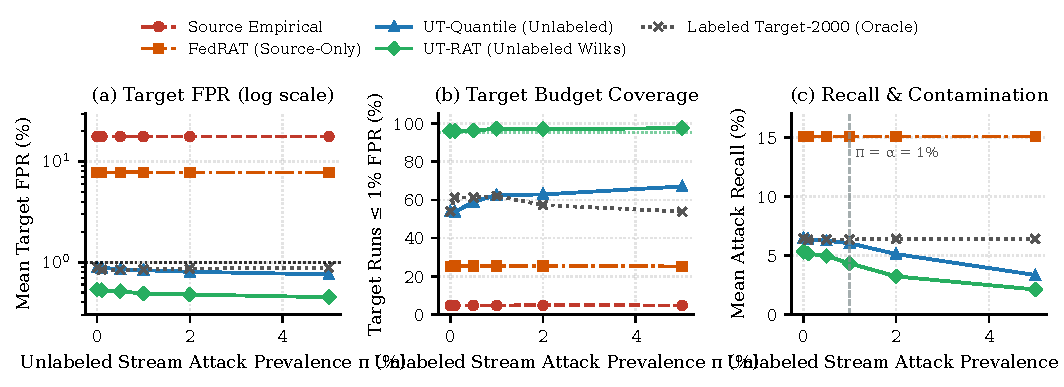
\includegraphics[width=.96\textwidth]{unsupervised_calibration.pdf}
\caption{Zero-target-label target-stream calibration across unlabeled attack prevalences $\pi\in[0\%,5\%]$ ($N_{\mathrm{cal}}=2{,}000$, $\alpha=1\%$, 300 native runs). (a)~Mean target FPR on a log scale; (b)~percentage of runs meeting the 1\% target budget; (c)~mean attack recall showing the attack-contamination boundary once $\pi$ exceeds $\alpha=1\%$.}\label{fig:utcal}\end{figure*}

Table~\ref{tab:utcal} and Fig.~\ref{fig:utcal} show that calibrating on an unlabeled target stream dramatically outperforms source-only policies without requiring target labels. At $\pi=1\%$, \texttt{UT-Quantile} reduces mean target FPR from 17.77\% (source empirical) and 7.81\% (FedRAT) to 0.83\%, raises target budget coverage to 62.53\%, cuts log FPR error to 0.98, and retains 6.04\% mean recall---95.0\% of the 6.36\% recall obtained with 2,000 \emph{labeled} benign target flows. For the strongest individual models at $\pi=1\%$, \texttt{UT-Quantile} attains 17.82\% recall at 0.90\% FPR (\texttt{LogisticRegression}), 14.26\% at 0.92\% FPR (\texttt{FedNova}), and 14.21\% at 0.93\% FPR (\texttt{SCAFFOLD}). Applying the Wilks tolerance rule to the unlabeled stream (\texttt{UT-RAT}) lifts target budget coverage from 25.53\% (FedRAT) to 97.13\% at 0.49\% mean target FPR (total alert rate 0.53\%). Across prevalences, Fig.~\ref{fig:utcal}(c) quantifies the attack-contamination trade-off: for $\pi\le\alpha$, unlabeled calibration closely tracks the labeled oracle; once $\pi>\alpha$ ($\pi=2\%$ and $5\%$), attacks inside the unlabeled stream push thresholds upward, preserving strict FPR control (0.76--0.80\%) while eroding recall from 6.47\% to 5.13\% and 3.36\%.

\subsection{Linear capacity, test-time BN adaptation, and tail-weighted losses}
\begin{table*}[t]\centering\footnotesize
\caption{Targeted federated extensions (80 runs across four held-out datasets and five seeds, matching Table~\ref{tab:primary}). Mean $\pm$ sample SD over four dataset means. The last two columns report zero-target-label \texttt{UT-Quantile} FPR/recall and \texttt{UT-RAT} coverage at $\pi=1\%$.}\label{tab:day2}
\setlength{\tabcolsep}{4pt}\begin{tabular}{lrrrrrrr}\toprule
Method & AUROC & pAUC$_{.01}$ & Locked FPR (\%) & Locked recall (\%) & Target-q. recall (\%) & UT-Q FPR / rec. (\%) & UT-RAT cov. (\%)\\\midrule
FedLogReg & \textbf{0.753} $\pm$ 0.170 & 0.528 $\pm$ 0.038 & \textbf{7.1} $\pm$ 6.1 & 35.6 $\pm$ 29.8 & \textbf{15.4} $\pm$ 23.3 & 0.93 / 11.0 & \textbf{100.0}\\
FedNova\_Tail & 0.689 $\pm$ 0.067 & \textbf{0.540} $\pm$ 0.063 & \textbf{7.1} $\pm$ 6.6 & 17.7 $\pm$ 8.1 & 12.2 $\pm$ 16.3 & 0.95 / \textbf{11.7} & 97.0\\
FedBN\_TTA & 0.691 $\pm$ 0.158 & 0.529 $\pm$ 0.021 & 36.4 $\pm$ 7.2 & 67.7 $\pm$ 20.8 & 8.4 $\pm$ 7.0 & \textbf{0.84} / 7.8 & 94.0\\
FedAvg\_Tail & 0.597 $\pm$ 0.143 & 0.507 $\pm$ 0.010 & 21.9 $\pm$ 6.3 & 35.4 $\pm$ 18.2 & 4.0 $\pm$ 4.6 & 0.81 / 3.4 & 99.0\\\bottomrule
\end{tabular}\end{table*}

\begin{figure*}[t]\centering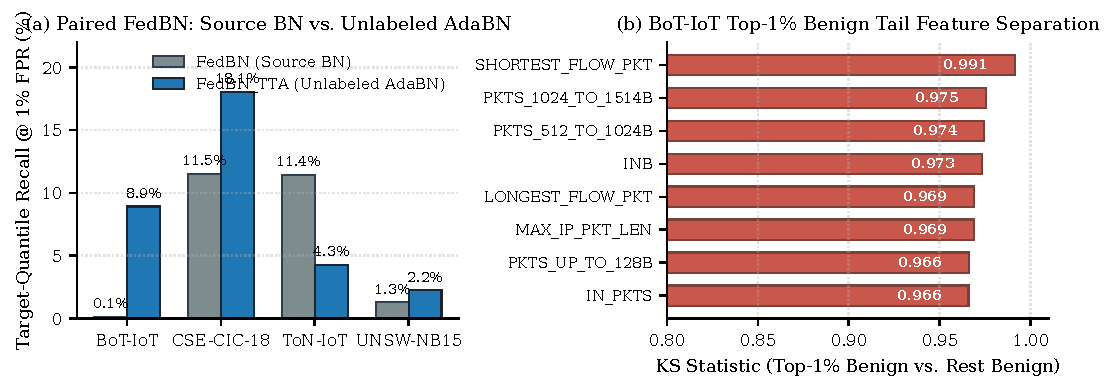
\includegraphics[width=.96\textwidth]{day2_extensions.pdf}
\caption{(a)~Paired \texttt{FedBN} target-quantile recall at 1\% FPR before and after zero-leakage unlabeled AdaBN (\texttt{FedBN\_TTA}) across the four held-out datasets; (b)~top eight NetFlow features separating the 109 consistent BoT-IoT top-1\% benign flows from the remaining benign traffic (KS statistic).}\label{fig:day2}\end{figure*}

Table~\ref{tab:day2} compares the four targeted federated extensions under the exact Table~\ref{tab:primary} protocol. Three clear patterns emerge:
\begin{itemize}
\item \textbf{Linear federated models dominate overall:} \texttt{FedLogReg} achieves the highest mean AUROC (\textbf{0.753}) of all 19 evaluated methods---surpassing \texttt{FedNova} (0.713), \texttt{FedAvg} (0.709), and centralized \texttt{LogisticRegression} (0.675)---alongside the lowest source-locked target FPR (7.1\%), the highest federated target-quantile recall (15.4\%, reaching 50.03\% on CSE-CIC-IDS2018), and 100.0\% target budget coverage under \texttt{UT-RAT}. Thus the low-FPR advantage of linear models observed in Table~\ref{tab:primary} is primarily an inductive-bias and regularization effect rather than a penalty of federated aggregation.
\item \textbf{Unlabeled TTA improves tail ranking but requires target calibration:} On identical trained weights and strictly disjoint evaluation splits (Fig.~\ref{fig:day2}(a)), \texttt{FedBN\_TTA} raises mean AUROC from 0.673 to 0.691, pAUC$_{.01}$ from 0.514 to 0.529, and target-quantile recall from 6.10\% to 8.37\% (+2.28\pp), improving three of four datasets---most notably breaking BoT-IoT's collapse from 0.13\% to \textbf{8.92\%} (+8.80\pp; AUROC 0.76 to 0.84) and lifting CSE-CIC-IDS2018 from 11.53\% to 18.05\% (+6.52\pp), while decreasing ToN-IoT (11.43\% to 4.26\%). Crucially, adapting BatchNorm shifts the target score scale, inflating source-locked FPR from 14.84\% to 36.40\% (+21.56\pp). Pairing \texttt{FedBN\_TTA} with zero-label \texttt{UT-Quantile} restores FPR to 0.84\% while preserving 7.8\% recall (94.0\% coverage under \texttt{UT-RAT}).
\item \textbf{Source-side tail weighting overfits source benign tails:} Replacing standard BCE with negative-tail focal weighting lowered \texttt{FedAvg} recall from 9.0\% to 4.0\% (AUROC 0.709 to 0.597; locked FPR 16.3\% to 21.9\%) and nudged \texttt{FedNova} from 14.8\% to 12.2\% (AUROC 0.713 to 0.689), indicating that aggressively penalizing high-scoring source benign flows overfits source-specific benign tails rather than generalizing to unseen target tails.
\end{itemize}

\section{Discussion}
\subsection{Threshold transfer and low-FPR discrimination}
At the source threshold, Random Forest detected nearly three fifths of target attacks while flagging nearly three tenths of benign flows. At the retrospective 1\% target budget, its recall fell below 1\%. For FedAvg on BoT-IoT, even an AUROC of 0.904 coexisted with almost zero recall after target-benign calibration. The correlation across method means ($r=-0.918$) links poor threshold transfer with weak tail ranking in these data. Both quantities depend on target benign scores; the association does not establish a causal mechanism.

\emph{BoT-IoT tail audit and attack-family concentration.} Earlier Euclidean-distance checks found that the highest-scoring 1\% of benign BoT-IoT flows (120 records per FedAvg seed) were actually farther from BoT-IoT attacks (median distance 14.37--16.75) than the remaining benign flows (4.27), ruling out simple attack-neighbor overlap. Feature-level attribution resolves this paradox (Fig.~\ref{fig:day2}(b)): 109 specific benign flows (92 appearing in 4 of 5 FedAvg seeds) are nearly disjoint from the remaining 11,684 benign flows (Kolmogorov--Smirnov statistics 0.949--0.991). Whereas 99\% of BoT-IoT benign records and BoT-IoT DDoS/DoS attacks are small 1--2 packet flows (medians: 44--112 \texttt{IN\_BYTES}, 40\,B \texttt{SHORTEST\_FLOW\_PKT}, 74\,B \texttt{LONGEST\_FLOW\_PKT}, TTL 0), these 109 heavy-hitter benign flows are large multi-hundred-packet, full-MTU transfers (medians: 746,807 \texttt{IN\_BYTES}, 809 \texttt{IN\_PKTS}, 427\,B \texttt{SHORTEST\_FLOW\_PKT}, 1,498\,B \texttt{LONGEST\_FLOW\_PKT}, 292 packets in 1024--1514\,B, TTL 127, and \texttt{SRC\_TO\_DST\_SECOND\_BYTES} $3.98\times 10^{15}$). Because those heavy-hitter benign flows sit at the extreme upper end of the score distribution, enforcing a 1\% target FPR pushes the threshold above nearly all small-packet BoT-IoT attacks, collapsing recall to 0.0\% until target-side BatchNorm statistics are adapted (\texttt{FedBN\_TTA}: 8.92\%). Across all four datasets, family-level 1\%-FPR recall is similarly concentrated: even top models (\texttt{LogisticRegression}, \texttt{FedNova}, \texttt{SCAFFOLD}) derive most of their low-FPR sensitivity from high-volume DDoS (78.7--92.2\% on CSE-CIC-IDS2018; 21.2--54.4\% on ToN-IoT) and ToN-IoT \texttt{password}/\texttt{injection} (9.9--33.1\%), whereas stealthier families (\texttt{Bot}, \texttt{Backdoor}, \texttt{Shellcode}, \texttt{Worms}, \texttt{Exploits}) remain at 0--4\% across all evaluated methods.

\subsection{Implications for federated optimization}
Federated optimization determines how clients train a shared model. Its objective need not preserve the ordering of rare, high-scoring benign flows on a new dataset. The local ensemble exceeded the federated group mean in target-quantile recall, while centralized logistic regression exceeded both. The pooled trees and neural baselines span quite different operating points. Training paradigm alone therefore gives little guidance about which detector will retain sensitivity under a strict false-alarm budget.

\subsection{Client heterogeneity and protocol sensitivity}
Relative to the mixed control, label skew improved both FedAvg's target-quantile recall and its partial AUROC under the tuned protocol. A change of decision threshold alone cannot explain an increase in a ranking metric. The earlier fixed-schedule experiment showed a different direction of effect. Several design choices changed between experiments, and the allocation variants inherited native hyperparameters. The reversal limits the generality of either finding.

\subsection{Limits of conservative thresholding}
FedRAT summarizes each source group's benign tail with a single scalar. This makes threshold exchange inexpensive when sites cannot share individual scores. Empirical budget coverage reached 100\% on the pooled source test but only 24.67\% on targets. A more conservative source threshold can sacrifice detections while still exceeding the target budget. The tolerance calculation offers no distribution-free protection under arbitrary target shift; scalar exchange alone provides neither differential privacy nor secure aggregation.

\subsection{Operational implications}
An operator needs two estimates: the alert volume at the available source threshold and the attack sensitivity that could be retained if the target budget were met. Target-informed calibration supplies a retrospective benchmark for the latter. Projecting alert volume additionally requires an assumed attack prevalence. At 1\% prevalence, the FedAvg estimate of roughly 404 detections among 16,505 alerts per 100,000 flows makes the operational cost visible even when recall on the balanced benchmark appears substantial.

\section{Scope and limitations}
The four source datasets are repeatedly reused across seeds, methods and policies. Between-dataset SD and paired contrasts quantify heterogeneity. Flow-level binomial intervals assume independent observations. Simulated allocations and shared normalization omit several operational privacy and communication costs. Calibration and alert extrapolation assume stable class-conditional rates. The raw-source release does not establish session or capture independence. Legacy Edge results used a different schema and training schedule; equal rounded rates do not establish identical predictions, model collapse or duplicate traffic. The effects of changed budgets, preprocessing and allocation cannot be separated by contrasting the two protocols. No temporal, independent external or tuned 14-family Edge result is claimed.

\section{Conclusion}
Across four held-out NetFlow datasets, source-calibrated thresholds frequently exceeded the target false-alarm budget, and restoring that budget retrospectively exposed weak low-FPR ranking for most models. Our extensions clarify what actually mitigates these failures: (1)~calibrating thresholds on an unlabeled target stream (\texttt{UT-Quantile} and \texttt{UT-RAT}) restores budget control without target labels (0.49--0.83\% target FPR, up to 97.1\% coverage) and retains 95\% of labeled-oracle recall whenever deployment prevalence stays below the nominal budget; (2)~regularized low-capacity federated models (\texttt{FedLogReg}) achieve the best overall AUROC (0.753), lowest source-locked FPR (7.1\%), and highest federated 1\%-FPR recall (15.4\%), whereas source-side tail-weighted losses overfit source benign tails; and (3)~unsupervised test-time BatchNorm adaptation (\texttt{FedBN\_TTA}) improves low-FPR tail ranking---breaking BoT-IoT's heavy-hitter benign collapse---but must be paired with unlabeled target calibration to prevent source-threshold FPR inflation. Independent external datasets and chronological holdouts remain necessary to assess broader deployment transfer.

\section*{Code and data availability}
Experiment code and reference outputs: \url{https://github.com/Fragoa/flids-benchmark}. Original NF-UQ-NIDS-v2 datasets: \url{https://staff.itee.uq.edu.au/marius/NIDS_datasets/}. The exact processed input digest and source digest are recorded in the repository. Raw flow data and the research checkpoint archive are separate inputs.
\appendices\section{Fixed-schedule experiments and statistical synthesis}
This appendix reports the earlier protocol. All operating rates, prevalence plots and budget comparisons below refer to that protocol. A row-ID-matched audit of the archived Edge predictions found that FedAvg and FedProx had exactly equal scores on only 0.38\% of records on average across 20 family--seed runs (median 0\%). Equal rounded operating rates therefore did not imply equal scores. The available predictions do not identify duplicate features or establish the cause of the DDoS-UDP tie. These estimates should not be substituted for the tuned results in Table~\ref{tab:primary}.
\subsection{Two Independent Holdout Tasks}
\textbf{Attack-family holdout (Exp.~1).} We scan the 2,219,201 records in the processed Edge-IIoTset CSV and form a capped 76,215-record, class-stratified reservoir. The input contains 30 numeric \emph{Safe-30} features selected to remove identifiers, raw ports, payload strings, and high-risk metadata. Four attack families are separately withheld: Port Scanning, DDoS-UDP, SQL injection, and Ransomware. Remaining attacks and benign traffic supply training and source validation. Each held-out family is then tested against a fixed benign subset. Five simulated clients use Dirichlet allocation (concentration $\alpha=0.5$). This is \emph{binary novelty detection} (attack versus benign), not open-set identification of a new attack class \cite{bendale2016}. The 64-bit full-feature-signature grouping prevents exact proxy-signature overlap in constructed splits but does not establish session independence.

\textbf{Source-dataset holdout (Exp.~2--6).} We scan all 75,987,976 records in NF-UQ-NIDS-v2 and sample up to 12,000 benign and 12,000 attack flows per component dataset (96,000 total). The 41 numeric NetFlow-v2 predictors exclude the source-dataset identifier and labels. We use four leave-one-source-dataset-out folds: NF-UNSW-NB15, NF-ToN-IoT, NF-BoT-IoT, and NF-CSE-CIC-IDS2018. In each fold, the other three source datasets form the training/validation pool; for the native federation each source corresponds to one simulated client. There is no target label, score, or example in scaling, fit, early model selection, or threshold choice. Because test samples are artificially 50\% positive, precision on those splits is \emph{not} a field estimate. Tests across these two feature schemas must not be compared as direct modality transfer.

\begin{table}[t]
\centering
\caption{Full-stream class counts in the four source datasets underlying NF-UQ-NIDS-v2. Training/testing instead use a balanced, capped reservoir.}
\label{tab:source}
\scriptsize\setlength{\tabcolsep}{3pt}
\begin{tabular}{@{}lrrr@{}}
\toprule
\textbf{Source dataset} & \textbf{Benign} & \textbf{Attack} & \textbf{Attack \%}\\
\midrule
NF-UNSW-NB15 & 2,295,222 & 95,053 & 3.98\\
NF-ToN-IoT & 6,099,469 & 10,841,027 & 63.99\\
NF-BoT-IoT & 135,037 & 37,628,460 & 99.64\\
NF-CSE-CIC-IDS2018 & 16,635,567 & 2,258,141 & 11.95\\
\midrule
\textbf{Total} & 25,165,295 & 50,822,681 & 66.88\\
\bottomrule
\end{tabular}
\end{table}

\subsection{Models, Budgets, and Controlled Variables}
Nine methods are evaluated on each of the two holdout tasks: centralized logistic regression, Random Forest \cite{breiman2001}, LightGBM \cite{ke2017}, and pooled MLP; the mean-score ensemble of independently trained local MLPs; and four federated MLPs (FedAvg, FedProx, FedAdam, FedYogi) \cite{mcmahan2017,li2020,reddi2021}. Centralized algorithms are \emph{not} FL implementations; a local ensemble incurs no federated \emph{training} aggregation but may incur operational score-fusion costs. Additional optimizer variants preserve the same target splits and source validation hashes as the five core methods, but their tuning budgets were not exhaustively optimized or benchmarked against external libraries.

Core MLP-based FL uses 30 communication rounds, one local epoch, Adam at learning rate $10^{-3}$, batch size 256, and a local-round sample cap (1024 on Edge-IIoTset, 512 on NF-UQ). FedProx uses $\mu=0.01$. Each configuration is repeated with seeds \{0, 42, 123, 2026, 3407\}. For the controlled Exp.~6 ablation, three clients participate each round, with architecture, held-out splits, rounds, and local step budget frozen. Client-size, label-prevalence, and domain-purity interventions are each compared against a mixed balanced control, with observed collateral changes in other marginals explicitly audited. In Exp.~5, participation is either two of three or all three clients. FL communication measures transmitted model-parameter payload only, excluding protocol, encryption, and real network transport overhead.

\subsection{Source-Locked Operating Points and Metrics}
Let $s(x)$ denote an attack score and let $V^0_{\mathrm{src}}$ be \emph{source-validation benign} scores. For target validation false-positive probability $q\in\{0.001,0.01,0.05\}$, a conservative empirical score quantile determines $\tau_q$; the classifier flags $s(x)>\tau_q$. The quantile is computed with a strict tie policy to avoid score-rounding threshold artifacts. We report separate target $\fpr$ and attack recall $\tp$: 
\begin{equation}
\fpr=\frac{FP}{FP+TN},\qquad \tp=\frac{TP}{TP+FN}.
\label{eq:fpr}
\end{equation}
Target-domain labels are used only for retrospective evaluation. In Exp.~3, we additionally compare the \emph{worst-source} benign quantile and an explicitly labeled \emph{target-oracle} quantile: the latter is an inaccessible, post-hoc diagnostic, never a deployment recommendation. Source-fitted Platt calibration and Brier score/expected calibration error (ECE) probe probability reliability \cite{guo2017,ovadia2019}.

For an \emph{assumed} attack prevalence $\pi$, Exp.~4 reweights measured conditional rates without retraining:
\begin{align}
\mathrm{PPV}(\pi)&=\frac{\pi\tp}{\pi\tp+(1-\pi)\fpr},\nonumber\\
A_{100k}&=10^5[\pi\tp+(1-\pi)\fpr].
\label{eq:ppv}
\end{align}
This prior-shift-only calculation requires conditional rates to remain fixed across prevalence scenarios. Alarm budgets $\{50,100,500,1000\}$ per 100,000 flows are selected using \emph{source} scores and evaluated on target predictions. A target-empirical threshold is not used to choose a deployable policy.

\subsection{Integrity and Statistical Protocol}
The NF-UQ audit enumerates class counts exactly from the full source stream, while fingerprint and data-quality checks examine 40,000 stratified records. It finds 475 extra duplicate-feature rows within this sample, no observed cross-source fingerprint group, and no binary-label conflict within inspected groups. Absence of a sampled collision is \emph{not} proof of full-data disjointness. The Edge-IIoTset 354,639-row signature audit finds 123 extra duplicates under a broad signature but many more collisions under Safe-30; 27 groups have binary-label conflicts when projected into Safe-30. Such collisions are information loss under feature reduction, not demonstrated source-label corruption. Source-dataset identity, capture identity, temporal independence, and row fingerprints are distinct concepts.

For statistics, we average seeds \emph{inside each held-out source or attack family}, then summarize the four distinct holdouts. Descriptive 95\% Student-$t$ intervals use four group means ($df=3$); thus they are wide, may exceed $[0,1]$, and are not presented as calibrated population uncertainty. Paired ablations match holdout and seed before subtraction. Four target domains do not support strong general-population or multiple-testing significance claims \cite{demsar2006}.

\subsection{Unseen Attack Families: High Recall Does Not Generalize Across Learners}
Table~\ref{tab:all9} reports the equal-family mean for the Edge task and equal-domain mean for the NF task, each at the 1\% \emph{source-validation} FPR target. Pooled LightGBM recalls 83.39\% of held-out attack samples on Edge-IIoTset with 0.91\% realized benign false positives in the sampled test. Random Forest reaches 72.46\% recall. FedAvg and FedProx each reach 15.04\%; FedAdam and FedYogi each reach 6.39\%. These comparisons are bounded by the chosen features, capacity, training schedule, and attack families; they do not show that FL fundamentally cannot detect novel attacks. Family-wise variability is substantial, so the mean must not be read as performance on an arbitrary new threat.

\begin{table}[t]
\centering
\caption{Nine-method synthesis at a \emph{nominal 1\% source-validation FPR target}. OS = unseen attack-family recall on Edge-IIoTset; CD = held-out NetFlow source dataset. All values are percentages except AUROC. CD FPR is \emph{actual target} FPR.}
\label{tab:all9}
\scriptsize\setlength{\tabcolsep}{2.6pt}
\begin{tabular}{@{}lrrrr@{}}
\toprule
\textbf{Model} & \textbf{OS rec.} & \textbf{CD rec.} & \textbf{CD FPR} & \textbf{CD AUC}\\
\midrule
Pooled LightGBM & \textbf{83.39} & 49.64 & 24.93 & .601\\
Random Forest & 72.46 & \textbf{62.45} & 31.53 & .634\\
Pooled MLP & 44.26 & 39.14 & 6.44 & .746\\
Logistic regression & 3.68 & 26.78 & 23.40 & .537\\
Local MLP ensemble & 14.59 & 20.61 & 2.46 & .729\\
FedAvg & 15.04 & 8.50 & 1.53 & .786\\
FedProx & 15.04 & 8.22 & 1.53 & .786\\
FedAdam & 6.39 & 5.00 & 2.38 & .528\\
FedYogi & 6.39 & 5.00 & 2.39 & .527\\
\bottomrule
\end{tabular}
\end{table}

\begin{table}[t]
\centering
\caption{Attack recall (\%) for individually held-out Edge-IIoTset families, averaged over five seeds at the 1\% source-validation FPR target. Each family is absent from training.}
\label{tab:attack_family}
\scriptsize\setlength{\tabcolsep}{3.5pt}
\begin{tabular}{@{}lrrrr@{}}
\toprule
\textbf{Held-out family} & \textbf{LGBM} & \textbf{RF} & \textbf{MLP} & \textbf{FedAvg}\\
\midrule
Port Scanning & 94.84 & 68.60 & 97.56 & 48.62\\
DDoS-UDP & 100.00 & 81.86 & 9.28 & 9.28\\
SQL injection & 72.79 & 72.69 & 15.92 & 0.01\\
Ransomware & 65.91 & 66.69 & 54.28 & 2.24\\
\bottomrule
\end{tabular}
\end{table}

The family-level view in Table~\ref{tab:attack_family} is more informative than the aggregate alone. Pooled MLP reaches 97.56\% on withheld Port Scanning but only 9.28\% on DDoS-UDP; the latter is recognized perfectly by pooled LightGBM in the same sampled holdout. Both FedAvg and FedProx almost entirely miss withheld SQL injection at the selected operating point. The result supports a statement about these fixed training schedules and attack families, rather than a claim about all novel attacks. Differences across family and model also caution against relying on a single reported novelty score.

\subsection{Unseen Domains: Operating-Point Reversal}
The ranking changes in the held-out NetFlow task (Table~\ref{tab:all9}). Random Forest has the highest mean cross-domain recall, 62.45\%, but triggers on 31.53\% of benign target traffic. Pooled LightGBM recalls 49.64\% with 24.93\% target FPR, despite its threshold being selected to aim for only 1\% \emph{on source validation}. Conversely, FedAvg's AUROC is 0.786, exceeding pooled LightGBM's 0.601, yet its operating recall is only 8.50\%. Thus, discrimination, source-threshold positioning, and realized target alarms are different properties. A higher raw target recall at 25--32\% false alarms is \emph{not} evidence of meeting a 1\% target-FPR requirement.



Across source datasets, a method can look nearly silent in one target and heavily over-alert in another. For example, with FedAvg the target FPR is approximately 0.07\% on NF-UNSW-NB15 but 4.64\% on NF-BoT-IoT; associated target attack recalls are only about 1.3\% and 23.9\%, respectively. The contrast is not solely an artifact of the number of random seeds; it exists between source datasets. When applying the same model to a new operational environment, threshold transfer warrants separate validation or explicit abstention/monitoring mechanisms.

\begin{table}[t]
\centering
\caption{Four target-source datasets at nominal 1\% source-validation FPR: mean target recall / actual target FPR (\%) over five seeds.}
\label{tab:per_domain}
\scriptsize\setlength{\tabcolsep}{3pt}
\begin{tabular}{@{}lrrr@{}}
\toprule
\textbf{Held-out target} & \textbf{RF} & \textbf{LightGBM} & \textbf{FedAvg}\\
\midrule
UNSW-NB15 & 24.68/37.82 & 18.63/28.92 & 1.33/0.07\\
ToN-IoT & 58.97/39.16 & 55.70/29.94 & 7.83/1.31\\
BoT-IoT & 77.41/13.90 & 84.22/10.69 & 23.90/4.64\\
CSE-CIC-2018 & 88.74/35.26 & 40.00/30.17 & 0.92/0.09\\
\bottomrule
\end{tabular}
\end{table}

As Table~\ref{tab:per_domain} shows, high raw recall of a centralized classifier often coincides with a target FPR far beyond the nominal one-percent goal. Random Forest exceeds 35\% FPR in three of the four targets, whereas under this schedule, FedAvg has much lower false-positive rates at the cost of failing to recognize most held-out attacks in two source domains. No single model dominates simultaneously in recall and realized FPR across all domains.

\subsection{Calibration, Feature Sensitivity, and Threshold Strategy}
Exp.~3 refits the five original methods on three feature sets: all 41 predictors, no source/destination port predictors, and no ports plus TTL features. At all features and 1\% source FPR target, pooled LightGBM yields 49.64\% recall / 24.93\% target FPR using a pooled-source threshold. A more conservative worst-source threshold yields 35.3\% / 16.1\%; FedAvg falls from 8.50\% / 1.53\% to 1.31\% / 0.43\%. The target-oracle point, included strictly for \emph{retrospective} diagnosis, reaches roughly 1\% target FPR at a different recall and is not deployable without target benign labels. These comparisons demonstrate an operational trade-off, not a universal superiority ranking of thresholds.

Source-fitted calibration also fails to transfer uniformly. For LightGBM, raw source ECE is 0.015 while raw target ECE rises to 0.326; source-fitted Platt scaling improves source ECE but worsens target ECE to 0.342. FedAvg changes from source ECE 0.098 to target ECE 0.228 (0.225 with source Platt scaling). Feature ablations further show that dropping ports can markedly reduce ranking quality: LightGBM average AUROC falls from 0.601 to 0.442, and FedAvg from 0.786 to 0.729. Removing potentially shortcut-prone inputs is not automatically a safe remedy because those inputs may also encode legitimate class information. Feature-level KS shift indicators (e.g., packet length, in-packet count, TTL, bytes) support distributional diagnostics but do not establish causality.

\subsection{Attack Prevalence and Alert Budgets}
Table~\ref{tab:budget} summarizes the earlier budget experiment; its scope is the fixed-schedule protocol. Operationally, Eq.~\eqref{eq:ppv} implies that false alarms can overwhelm true detections even if recall looks respectable. At an \emph{assumed} 1\% attack prevalence with the unchanged five-core-model conditional rates, the mean expected precision is 2.87\% for pooled LightGBM, 6.07\% for pooled MLP, 11.11\% for the local ensemble, 10.84\% for FedAvg, and 10.47\% for FedProx. In the same scenario, expected alerts per 100,000 flows are 25,176, 6,769, 2,646, 1,599, and 1,601, respectively (Fig.~\ref{fig:alerts}). These are \emph{reweighted expectations}, not production traffic counts. The original source prevalence is also not necessarily a genuine field attack rate because the corpora were collected for benchmark purposes.

\begin{figure*}[t]
\centering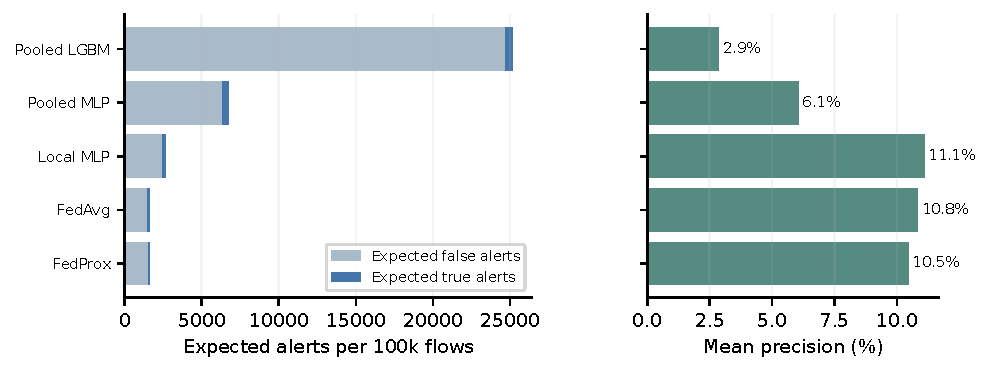
\includegraphics[width=.96\textwidth]{prevalence_operational.pdf}
\caption{Operational implications for the \emph{assumed} 1\% attack-prevalence scenario at source-validation FPR target 1\%, in Exp.~4 using Exp.~3 conditional scores. Left: expected true/false alerts per 100,000 flows. Right: mean per-run PPV (precision), which need not equal the ratio of aggregated means. No deployment measurements or new training are involved.}
\label{fig:alerts}
\end{figure*}

When the source score distribution is used to set a budget of 500 alerts per 100,000 flows, the average target alarms for pooled MLP are 1,110, with the budget violated in 45\% of domain--seed cases. Under the same procedure, LightGBM produces only about 10 alerts on average but recalls roughly 0.05\% of attacks. Meeting an alert cap by suppressing almost all attacks is not a successful operational trade-off. At a 1,000-alert budget, pooled MLP reaches approximately 28.8\% recall while violating the cap in 65\% of cases. A deployable system must assess both violations \emph{and} missed detections.

\begin{table}[t]
\centering
\caption{Fixed-schedule budget-transfer diagnostic (Exp.~4). Scenario assumes 1\% attack prevalence; budget set on source scores only. A ``violation'' is any target run exceeding the budget.}
\label{tab:budget}
\scriptsize\setlength{\tabcolsep}{3.2pt}
\begin{tabular}{@{}lrrr@{}}
\toprule
\textbf{Model} & \textbf{Budget} & \textbf{Target alerts} & \textbf{Viol. \%}\\
\midrule
LightGBM & 500 & 10 & 0\\
Pooled MLP & 500 & 1,110 & 45\\
Local MLP & 500 & 563 & 40\\
FedAvg & 500 & 170 & 10\\
FedProx & 500 & 147 & 5\\
Pooled MLP & 1,000 & 3,454 & 65\\
FedAvg & 1,000 & 1,015 & 35\\
\bottomrule
\end{tabular}
\end{table}

\subsection{Client Participation and Factor-Isolated Heterogeneity}
Exp.~5 varies three client allocations (native source-dataset clients, quantity-skew mixing, label-skew mixing) and participation of two or three clients. Native-domain FedAvg recall increases from 5.97\% with two participants to 8.50\% with three; the parameter payload increases from roughly 2.20 to 3.30\,MiB. This is a simulated model-update budget, not real end-to-end network cost. However, Exp.~5's quantity-skew case changes \emph{both} client size and source-domain mixing; the larger recall for that condition cannot be attributed to client quantity alone.

Exp.~6 corrects that confound with a matched mixed-control design and separate marginal interventions (Fig.~\ref{fig:hetero}). At a 1\% source validation FPR target, FedAvg mean recall drops from 29.37\% (control) to 3.43\% under severe label skew and to 8.50\% under severe source-domain separation. In contrast, strong quantity skew yields 26.38\%. Actual target FPR also changes: 3.14\% in control, 1.06\% in severe label skew, and 1.53\% in severe domain separation. Hence reduced recall partly co-occurs with suppressed alarms. Notably, source-domain separation preserves mean AUROC near 0.786 even as operating recall collapses, consistent with score-threshold transfer problems rather than a universal loss of ranking capability. The independent comparison unit remains the four held-out datasets, not the 20 paired seed runs.

\begin{figure*}[t]
\centering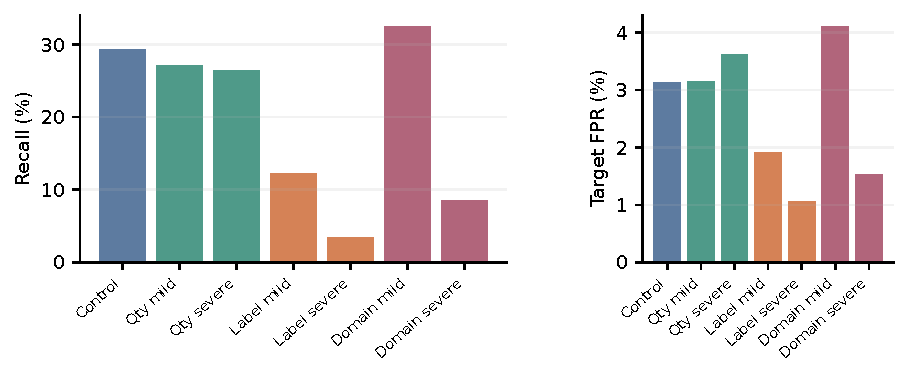
\includegraphics[width=.92\textwidth]{heterogeneity.pdf}
\caption{FedAvg controlled allocation ablation (Exp.~6), averaged across four held-out datasets and five seeds. Client quantity, binary-label skew, and source-domain purity are varied separately relative to the mixed control; target FPR is reported alongside recall. ``Severe'' indicates the study's preset intervention magnitude, not an externally standardized severity level.}
\label{fig:hetero}
\end{figure*}

FedProx tracks FedAvg closely: the mean FedProx-minus-FedAvg recall difference across the controlled scenarios is approximately +0.08 percentage points, with nearly identical communication payload. In Exp.~5 its average difference is about --0.12 percentage points. For $\mu=0.01$, the results show no persuasive consistent improvement from the proximal penalty, but broader optimizer tuning and alternative architectures remain untested. FedAdam and FedYogi were only added to the two primary holdout benchmarks, not retrospectively to Exps.~3--6; this limitation is made explicit rather than implying nine-model support for every diagnostic.

\subsection{Across-Holdout Uncertainty and Reproducibility}
The principal statistical synthesis contains 180 model trainings and 540 threshold-specific operating points on each of the two nine-model tracks, plus 300 trainings in Exp.~3, 240 runs in Exp.~5, and 280 runs in Exp.~6; Exp.~4 only replays existing predictions. For each stage we retain experiment configuration, source-data and split provenance where available, seed-level operating metrics, and run-completion gates. The two extra federated optimizers and the two extra classical methods were added only to Exps.~1--2 and matched against the original source-validation and test split digests. We do not conceal this asymmetry by calling the later five-method calibration experiment a nine-method experiment.

Ninety-five-percent domain-level descriptive intervals are particularly imprecise for quantities dominated by domain variation: the between-dataset recall contrast is far larger than typical seed-to-seed changes. Paired differences preserve the matching, but comparisons should still be interpreted as observations over four explicit source environments. This is why the primary results emphasize numerical effect sizes, simultaneous FPR reporting, and sign consistency rather than a long list of superficially significant $p$-values. For future replication, the evaluated data source versions, selection seeds, source-only validation split definitions, and preprocessing recipes should be archived together with the manuscript and public scripts; the current saved output set is sufficient for checking the reported aggregate statistics without re-running the 76-million-record scan.

\bibliographystyle{IEEEtran}
\bibliography{references}
% Replace the three reserved blocks with the approved bios and photographs.
% Each unsplittable block reserves 1.65 inches of column height plus separation.
\newcommand{\reservedbio}[1]{\par\noindent\begin{minipage}[t][1.65in][t]{\columnwidth}
\noindent\begin{minipage}[t]{1.03in}\vspace{0pt}\fbox{\parbox[c][1.20in][c]{.90in}{\centering\footnotesize Author photo}}\end{minipage}\hfill
\begin{minipage}[t]{\dimexpr\columnwidth-1.16in\relax}\vspace{0pt}\textbf{#1}\\[3pt]\footnotesize Biography reserved for the camera-ready manuscript.\end{minipage}
\end{minipage}\par\medskip}
\section*{Author Biographies}
\reservedbio{First Author}
\reservedbio{Second Author}
\reservedbio{Third Author}
\end{document}